\section{每个SM分配的活跃线程块详解}

\subsection{引言：核心概念与硬件限制表}

欢迎大家。今天的文章聚焦于GPU性能分析中的一个基本概念，即每个SM分配的活跃块（Active Blocks perSM
）。这个术语不仅与占用率同等重要，而且它直接影响占用率或GPU利用率。

要完全理解这个术语，必须将注意力转向这张表格。这张展示的表格是我从A100GPU白皮书中拿来的，该表格显示了Ampere
架构的硬件限制或约束。我不会涵盖表格中的所有行，为了今天的目的我将只重点介绍四个关键行。这意味着在任何给定时间，每个SM
上不能超过32个块同时运行或并发运行。


\begin{figure}
    \centering
    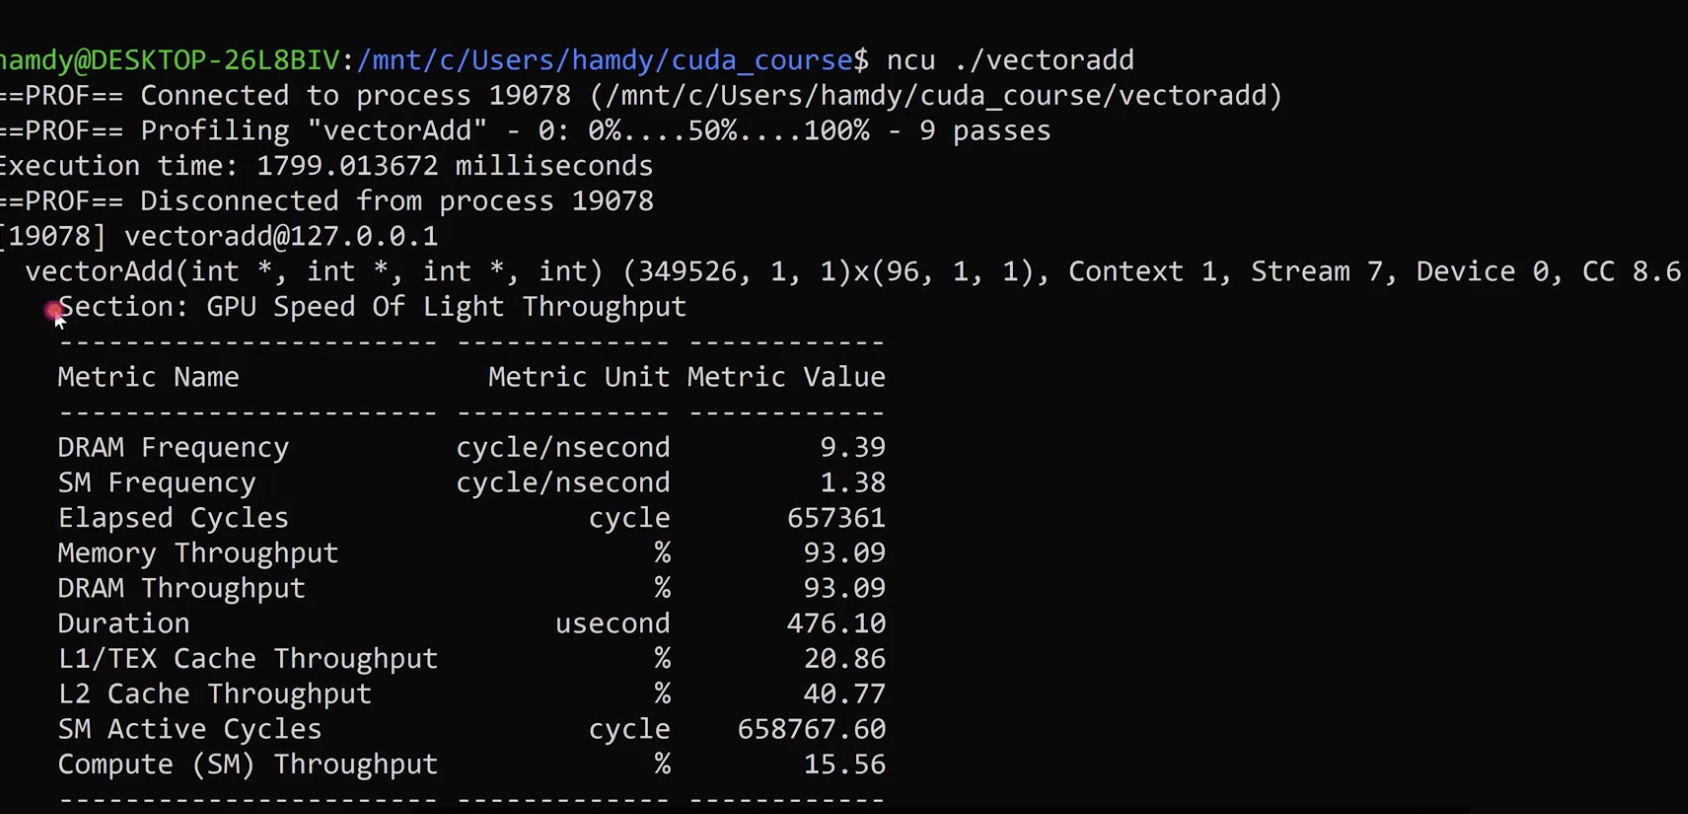
\includegraphics[width=0.75\linewidth]{resources/cuda-095.png}
    \caption{}
    \label{fig:placeholder}
\end{figure}


\subsection{四个关键硬件限制}

\subsection{每个SM的最大线程块数}

本文章中要检查的第一行是每个SM的最大线程块数，在这种情况下其值为32个块。最大值是32个块。

\subsection{每个SM的最大Warp数}

我今天想检查的第二行呈现了每个SM的最大Warp数，即单个SM上可以同时执行的最大Warp数。对于A100GPU，这个限
制是每个SM64个Warp。这意味着无论每个SM分配的块数是最大值32个块还是更少，这些块中所有Warp的总和不能超过每
个SM的最大Warp数，即64。

这是这里的主要关键点：\textbf{Warp数限制控制着每个SM可以分配多少个活跃块}。我们知道最大值是每个SM32个
块，但应用程序可能使用少于32个块，这取决于Warp数限制。我希望你把这句话记在心里，永远记住这句话。

然而如果每个块包含4个Warp，那么32个块的Warp总数将是128个Warp。为了理解这一点，让我们考虑一个例子：应用
程序每个SM分配32个块，这等于表格中提到的每个SM最大块数。但这个值128个Warp超过了表格中规定的Warp数限制，
编译器将尝试解决这个问题。

根据表格该值不应超过64个Warp，编译器会介入遵循以下逻辑：编译器理解每个SM最多可以利用32个块，然而如果每个块由4
个Warp组成，那么总的Warp数将是128。这超过了可接受的Warp数限制（而不是块限制）。编译器将决定将活跃块的数量
从32减少到16。经过这个调整，总的Warp数将变成$16 \times 4 = 64$ 个Warp。这个值落在可接受的
范围内并且没有超过Warp数限制。

\subsection{块限制Warp数（Block Limit Warp）}

如何控制每个SM分配的活跃块？这个例子揭示了一个关键概念，称为“块限制Warp数”（Block LimitWarp）。正
如这张我从NsightCompute工具分析中获取的图片所示，很明显“块限制Warp数”这个术语出现在占用率部分。这强调
了我之前在占用率文章中提到的关于占用率与每个SM分配的活跃块之间关系的观点。这个例子表明，尽管最大块限制是每个SM32个
块，但最终每个SM分配的块数受Warp数限制的约束。

\subsection{全局块分配与并发块的区别}

我想提一个关键点：可以在整个GPU上运行的最大块数非常大，可能达到数百万。你可以通过之前讨论过的CUDA运行时API来检
查这个限制。这个巨大的数字需要分布在数十个SM上。在A100GPU中我们有108个SM，这意味着有可能为每个SM分配超过
1000个块。然而这里的关键问题是：这1000个块中有多少个可以在一个SM上\textbf{并发运行}？

当我们提到每个SM 32个块的限制时，并不意味着只能分配32个块；相反意味着你可以分配超过32个，但只有32个或更少的块
会同时运行或并发运行。

\subsection{寄存器限制与寄存器溢出}

同样的原则适用于每个SM的最大寄存器数。A100 GPU中的最大值超过65000。

例如，考虑一个应用程序利用一个块，每个SM块大小为1024个线程。我们每个SM只有一个块，然而表格设定的限制仅为65536。如果每个线程需要100个寄存器，那么每个SM所需的总寄存器数将是$1024 \times 100 = 102400$
个寄存器，超过了允许的最大限制。

在这种情况下，我们不能通过减少每个SM的块数来解决这个问题，因为应用程序每个SM只利用一个块。你可以减少每个块的线程数来
解决这个问题，但如果你不这样做，那么所需的寄存器将超过允许的最大限制。

\textbf{寄存器溢出}（Register Spilling）会导致性能下降，这是因为本地内存比普通寄存器慢。这将导
致使用本地内存来存储这些寄存器的值。检查你的应用程序是否过度依赖寄存器溢出是至关重要的，你应该寻求改进应用程序的方法来缓
解这个问题。

\subsection{寄存器限制计算示例}

在这个例子中，我们需要计算每个SM分配的活跃块数。设块大小为512个线程（可配置参数），每个线程需要16个寄存器（取决于
应用程序代码，不在我们控制范围内）。

每个块所需的总寄存器数：$512 \times 16 = 8192$ 个寄存器。

在寄存器限制为每个SM 65536个寄存器的情况下，可以并发运行的最大块数
： \[\left\lfloor \frac{65536}{8192} \right\rfloor =
8 \text{ 个块}\]

这意味着尽管规定的块限制是每个SM 32个块，但在寄存器限制下将只选择8个块来并发运行。

\subsection{四重限制取最小值原则}

同样的原则适用于可用的Warp数（Warp限制）、可用的寄存器数（寄存器限制），以及表格最后一行的共享内存限制。虽然我现
在不会深入探讨共享内存约束的细节，但我们将在后面更深入地探讨这个主题。

我想解释最后一个例子，以说明Warp限制、寄存器限制和共享内存限制对每个SM分配的活跃块的影响。“分配的活跃块”指的是这
些块中有多少个可以\textbf{并发运行}，你可以为每个SM分配数百或数千个块，但并发数受限。

假设以下条件：
\begin{itemize}
    \item \textbf{块限制Warp数}: 4个块（如果使用超过4个块，将超过Warp数限制）
    \item \textbf{块寄存器限制}: 8个块
    \item \textbf{块共享内存限制}: 16个块
    \item \textbf{硬件最大块限制}: 32个块
\end{itemize}

在这四个值中，NVCC编译器将选择它们中\textbf{最小的值}。尽管块限制是32，寄存器限制是8，共享内存限制是16
，但Warp限制约束会超越它们，规定最多只能并发运行4个块。寄存器说可以运行8个，但Warp限制说不能运行超过4个。最终
值将取最小的那个值。

我想你现在可能明白了为什么我们在计算理论占用率时要取最小值。这就是为什么你需要理解“每个SM分配的活跃块”这个术语，以便
能够理解为什么在分析应用程序时要在这四个值中选择最小值。

\subsection{Nsight Compute实测验证：RTX 3090}

\begin{figure}
    \centering
    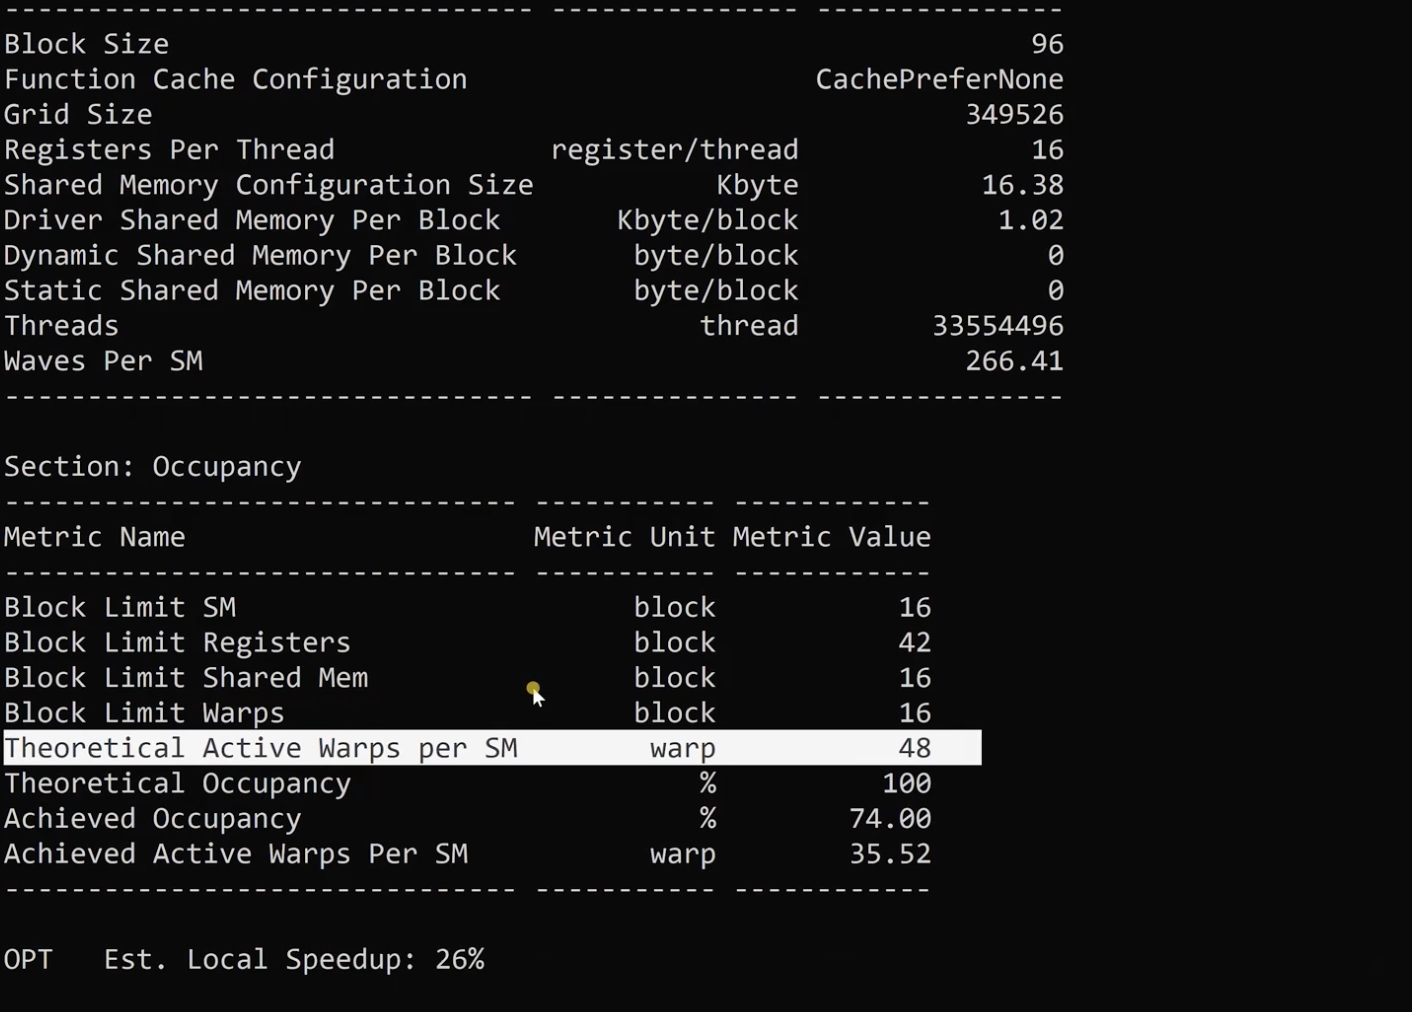
\includegraphics[width=0.75\linewidth]{resources/cuda-096.png}
    \caption{}
    \label{fig:placeholder}
\end{figure}

现在让我们再次分析向量加法应用程序。输入 \texttt{ncu ./vector\_add}（即NsightCompute）。如你所见，我们有三个部分：GPU Speed of Light、LaunchStatistics和Occupan

cy。我们需要的是占用率部分。


在这个部分内，前四个度量指标就是我们今天研究过的：
\begin{itemize}
    \item \textbf{块限制Warp数}: 16个块
    \item \textbf{块共享内存限制}: 对应值
    \item \textbf{块寄存器限制}: 42个块（今天影响较小）
    \item \textbf{硬件最大块限制}: 32个块
\end{itemize}

这四个值中的最小值是16。你可能想知道为什么是16而不是32？因为这里我是在RTX 3090GPU上解释，而不是A100
GPU。让我通过 \texttt{nvidia-smi}来检查一下，或者使用运行时API检查每个SM的最大分配活跃块数。

在这种情况下，每个SM分配的活跃块数是16个块，这就是我们用于理论占用率计算的值，我们不能并发运行超过16个块。

\subsection{理论占用率100\%的验证}

例如这里的理论占用率是100\%。为什么是100\%？我们知道块大小是96。让我们进行上一个文章中已经做过的相同计算：

\[\text{每块Warp数} = \frac{96}{32} = 3 \text{ 个Warp}\]

RTX 3090中每个SM的最大Warp数是48（我在占用率文章中解释过这个值）。如果我们有3个Warp乘以从四个值中得
到的最小分配活跃块数16：\[3 \times 16 = 48 \text{ 个Warp}\]

而在我的应用程序中我们利用了48个Warp。如果每个SM的最大活跃Warp数是48，那么：\[\text{理论占用率}
= \frac{48}{48} \times 100\% = 100\%\]

这就是为什么理论占用率是100\%。这只是理解这些参数的影响及其含义的一个例子，因为如果我们用最大值除以应用程序中利用的
值，百分比将是100\%。

